% Column generation: what the benchmark measured since last week, and where to go next. For the colleagues.
% Build: python make_data.py && latexmk -pdf slides.tex
\documentclass[aspectratio=169]{beamer}

\usetheme{Boadilla}
\usecolortheme{default}

\usepackage[T1]{fontenc}
\usepackage[utf8]{inputenc}
\usepackage{booktabs}
\usepackage{array}
\usepackage{tikz}
\usetikzlibrary{positioning,arrows.meta,fit}
\usepackage{pgfplots}
\usepackage{pgfplotstable}
\pgfplotsset{compat=1.18}

\definecolor{GLBlue}{RGB}{22,63,95}
\definecolor{GLGray}{RGB}{96,104,114}
\definecolor{GLLight}{RGB}{232,240,248}
\definecolor{GLOrange}{RGB}{214,110,30}
\definecolor{GLRed}{RGB}{190,40,40}
\definecolor{GLGreen}{RGB}{40,120,60}

\setbeamercolor{normal text}{fg=black,bg=white}
\setbeamercolor{title}{fg=GLBlue}
\setbeamercolor{subtitle}{fg=GLGray}
\setbeamercolor{frametitle}{fg=GLBlue,bg=GLBlue!6}
\setbeamercolor{titlelike}{fg=GLBlue}
\setbeamercolor{author}{fg=GLGray}
\setbeamercolor{date}{fg=GLGray}
\setbeamercolor{structure}{fg=GLBlue}
\setbeamercolor{itemize item}{fg=GLBlue}
\setbeamercolor{itemize subitem}{fg=GLGray}
\setbeamercolor{block title}{fg=white,bg=GLBlue}
\setbeamercolor{block body}{fg=black,bg=GLLight}

\setbeamerfont{title}{size=\LARGE,series=\bfseries}
\setbeamerfont{subtitle}{size=\normalsize}
\setbeamerfont{frametitle}{size=\Large,series=\bfseries}

\setbeamertemplate{navigation symbols}{}
\setbeamertemplate{headline}{}
\setbeamertemplate{footline}[frame number]
\setbeamertemplate{itemize subitem}[triangle]

\tikzset{
  box/.style={draw=GLBlue, fill=GLLight, rounded corners=2pt, align=center, font=\small,
    minimum height=2.2em, inner sep=4pt},
  later/.style={box, dashed, draw=GLGray, fill=white, text=GLGray},
  flow/.style={-{Stealth[length=5pt]}, GLBlue, thick},
}

\newcommand{\done}{\textcolor{GLGreen}{\textbf{done}}}
\newcommand{\todo}{\textcolor{GLGray}{next}}

\title{Column generation: the benchmark at work}
\subtitle{What it measured since last week, and where to go next}
\author{Leo Marbehan}
\date{November 2026}

\begin{document}

\begin{frame}[plain]
  \titlepage
\end{frame}

%--------------------------------------------------------------
\begin{frame}{Since last week}
  Last week: the benchmark's design, and the list of tasks it would serve.

  \vspace{0.4em}
  \small
  \begin{tabular}{@{}>{\raggedright\arraybackslash}p{0.38\textwidth}>{\raggedright\arraybackslash}p{0.08\textwidth}
      >{\raggedright\arraybackslash}p{0.46\textwidth}@{}}
    \toprule
    task & status & what came of it \\
    \midrule
    the benchmark: runners, benchmark, summary & \done & three runners, a comparison script, in review \\
    Python VRP example on the package & \done & same LP, never slower; in review \\
    C++ VRP example on the C++ example layer & \done & same LP, never slower; the \texttt{cpp-native} runner \\
    many cheap iterations & \done & 399 runs on the quiet machine: the three layers equal \\
    ng-routes & \todo & checked that they work; the comparison is next \\
    the engine's newer features & \todo & after ng-routes \\
    \bottomrule
  \end{tabular}

  \vspace{0.6em}
  \begin{itemize}\small
    \item Every number in this talk comes from the benchmark or from scripts kept next to its results.
    \item A home server now runs the long measurements (next slide).
  \end{itemize}
\end{frame}

%--------------------------------------------------------------
\begin{frame}{The benchmark as built}
  \begin{columns}[T]
    \begin{column}{0.52\textwidth}
      \centering
      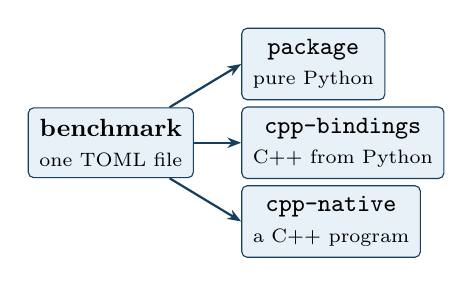
\begin{tikzpicture}[node distance=0.35cm and 0.6cm]
        \node[box] (bench) {\textbf{benchmark}\\\scriptsize one TOML file};
        \node[box, right=of bench, yshift=1.0cm] (package) {\texttt{package}\\\scriptsize pure Python};
        \node[box, right=of bench] (bindings) {\texttt{cpp-bindings}\\\scriptsize C++ from Python};
        \node[box, right=of bench, yshift=-1.0cm] (native) {\texttt{cpp-native}\\\scriptsize a C++ program};
        \draw[flow] (bench) -- (package.west);
        \draw[flow] (bench) -- (bindings.west);
        \draw[flow] (bench) -- (native.west);
      \end{tikzpicture}
    \end{column}
    \begin{column}{0.44\textwidth}
      \begin{itemize}\small
        \item the three runners give the \textbf{same LP, iterations and columns} (a test checks it)
        \item masters: highspy and gurobipy from Python; HiGHS and Gurobi in C++
        \item summary per case, and a comparison of two cases with our equivalence rule
        \item about 420 tests
      \end{itemize}
    \end{column}
  \end{columns}

  \vspace{0.6em}
  \begin{block}{A quiet machine for timings}
    \small An old laptop at home, idle, one run at a time. Run-to-run spread \textbf{1--3\,\%}, against 2--13\,\%
    on my desktop (up to 126\,\% on a bad case). It is slower, but it is the timing reference now.
  \end{block}
\end{frame}

%--------------------------------------------------------------
\begin{frame}{The Python VRP example, ported to the package}
  \small Home server, master over Gurobi on both sides (the old example through python-mip), one route per
  customer to start. Equivalence rule: same LP, time within max(5\,\%, 0.25\,s).

  \vspace{0.3em}
  \footnotesize
  \begin{tabular}{@{}lrrrrrl@{}}
    \toprule
    instance & LP & iterations old / new & solve s old & solve s new & difference & rule \\
    \midrule
    C101\_25 & 191.81 & 21 / 21 & 0.22 & 0.10 & $-0.12$ s & pass \\
    R201\_25 & 449.66 & 16 / 15 & 1.46 & 1.22 & $-0.24$ s & pass \\
    C101\_50 & 363.25 & 43--55 / 49 & 0.65 & 0.45 & $-0.20$ s & pass \\
    R201\_50 & 756.34 & 30 / 28 & 22.6 & 21.2 & $-6$\,\% & pass \\
    C201 & 591.56 & 165--184 / 344 & 64.7 & 64.2 & $-1$\,\% & pass \\
    R201 & 1084.99 & 42--46 / 43 & 3,302 & 2,235 & $\mathbf{-32}$\,\% & pass \\
    \bottomrule
  \end{tabular}

  \vspace{0.5em}
  \begin{itemize}\small
    \item \textbf{9 instances out of 9}: same LP, the package never slower. Peak memory lower (R201 about 295 MB
      against 510 MB).
    \item The package repeats exactly; the old example takes another path from one run to the next.
  \end{itemize}
\end{frame}

%--------------------------------------------------------------
\begin{frame}{The C++ VRP example, ported to the C++ example layer}
  \small Laptop, idle, Gurobi's C++ API on both sides, one route per customer to start.

  \vspace{0.3em}
  \footnotesize
  \begin{tabular}{@{}lrrrrrl@{}}
    \toprule
    instance & LP & iterations old / new & solve s old & solve s new & difference & rule \\
    \midrule
    C101\_25 & 191.81 & 22 / 29 & 0.036 & 0.043 & $+0.007$ s & pass \\
    R201\_25 & 449.66 & 22 / 12 & 0.49 & 0.30 & $-0.20$ s & pass \\
    R201\_50 & 756.34 & 45 / 26 & 15.4 & 4.8 & $-69$\,\% & pass \\
    C201 & 591.56 & 245 / 233 & 26.8 & 16.8 & $-37$\,\% & pass \\
    R201 & 1084.99 & 112 / 47 & 5,721 & 1,253 & $\mathbf{-78}$\,\% & pass \\
    \bottomrule
  \end{tabular}

  \vspace{0.5em}
  \begin{itemize}\small
    \item \textbf{9 instances out of 9} pass. The program is also the benchmark's \texttt{cpp-native} runner.
    \item The engine's own benchmarks (per-algorithm timings, Boost) left the example; they come back as options
      of the benchmark.
  \end{itemize}
\end{frame}

%--------------------------------------------------------------
\begin{frame}{Where the gains come from}
  Same duals given to both sides at every iteration (a replay), the master left out.

  \vspace{0.4em}
  \begin{columns}[T]
    \begin{column}{0.48\textwidth}
      \textbf{The search}
      \begin{itemize}\small
        \item the same paths at every iteration, C++ and Python
        \item C++: 0.97--1.00 of the old time per iteration
      \end{itemize}

      \vspace{0.3em}
      \textbf{The layers' own work}
      \begin{itemize}\small
        \item Python: the package is \textbf{3--7 times cheaper per column} than the old example (no
          dictionaries of duals, no path objects)
        \item C++: adding columns is the one slower part, and grows with the master (C201: 15 against 1.3\,\textmu s
          a column)
      \end{itemize}
    \end{column}
    \begin{column}{0.48\textwidth}
      \begin{block}{So}
        \small
        \begin{itemize}
          \item the big gains (R201: $-32$\,\%, $-78$\,\%) are the \textbf{path}: fewer iterations, fewer columns
          \item the code itself is as fast or faster, except the C++ column adds
          \item nothing that would hold back the ports
        \end{itemize}
      \end{block}
    \end{column}
  \end{columns}
\end{frame}

%--------------------------------------------------------------
\begin{frame}{The three layers, with many cheap iterations}
  \begin{columns}[T]
    \begin{column}{0.5\textwidth}
      \begin{tikzpicture}
        \begin{semilogxaxis}[
            width=\linewidth, height=5.6cm,
            xlabel={C++ from Python: ms per iteration},
            ylabel={pure Python: extra, \% of an iteration},
            xmin=1, xmax=300, ymin=-5, ymax=80,
            tick label style={font=\scriptsize}, label style={font=\scriptsize},
            legend style={font=\scriptsize, at={(0.97,0.97)}, anchor=north east},
          ]
          \addplot[only marks, mark=*, mark size=1.8pt, GLOrange] table[x=bindings_ms, y=extra_percent]
            {highspy.dat};
          \addlegendentry{highspy}
          \addplot[only marks, mark=square*, mark size=1.6pt, GLBlue] table[x=bindings_ms, y=extra_percent]
            {gurobipy.dat};
          \addlegendentry{gurobipy}
          \addplot[GLGray, dashed, domain=1:300] {5};
        \end{semilogxaxis}
      \end{tikzpicture}
    \end{column}
    \begin{column}{0.46\textwidth}
      \small Home server, 16 instances (25, 50, 100 customers), exact pricing, 3 rounds: 336 runs (and 63 more
      with tabu stages, same conclusions).
      \begin{itemize}\small
        \item the three layers give the \textbf{same results} everywhere (one Gurobi path apart)
        \item pure Python against C++ from Python: \textbf{the rule passes on every case}
        \item per iteration it costs about \textbf{1--2.5 ms more over highspy}, 0.2--1.6 ms over gurobipy
          (iterations under 100 ms)
        \item above 5\,\% (dashed line) only when an iteration takes less than about 30 ms
      \end{itemize}
    \end{column}
  \end{columns}
\end{frame}

%--------------------------------------------------------------
\begin{frame}{Found on the way}
  \begin{itemize}\small
    \item \textbf{Preprocessing in the pricer}: on by default, it costs 0.5--3 ms a search and never paid off on
      these instances, ng-routes included. It stays on, and can be turned off.
    \item \textbf{ng-routes work} through the layers (checked with 8 and 16 neighbours).
    \item \textbf{An artificial start can stall}: on R202\_50 the first exact search on the big-M duals takes a
      whole hour. A start with one route per customer, or a heuristic stage first, avoids it.
    \item \textbf{The search called from Python} is 5--6\,\% slower than from a C++ program with tabu stages;
      cause not measured.
    \item \textbf{Adding columns} through gurobipy costs 20--80\,\% more than through python-mip, and the C++
      layer's column adds slow down as the master grows.
    \item \textbf{Truncating the search} (stopping after 1 or 5 columns) does not make iterations cheap on R2
      instances: 70--80 ms a search either way.
  \end{itemize}

  \vspace{0.3em}
  \small\textcolor{GLGray}{The last three could become issues.}
\end{frame}

%--------------------------------------------------------------
\begin{frame}{Next: finishing the first phase}
  Each a benchmark option, measured the same way.

  \vspace{0.4em}
  \small
  \begin{tabular}{@{}>{\raggedright\arraybackslash}p{0.34\textwidth}>{\raggedright\arraybackslash}p{0.6\textwidth}@{}}
    \toprule
    task & what it gives \\
    \midrule
    ng-routes & an ng size option; LP values against the ng comparison program \\
    the engine's newer features & the bidirectional search and its options as stage parameters \\
    the engine benchmarks' features & bucket containers, Boost's search in the C++ runner \\
    pricing on one dual sequence & every algorithm on the same duals: time per search, columns found \\
    presets & the pricing setups the benchmark ships, chosen together \\
    plots & series, box plots, performance profiles, convergence curves \\
    the highspy path (optional) & the pure layer's extra 1--2.5 ms per iteration over highspy \\
    \bottomrule
  \end{tabular}
\end{frame}

%--------------------------------------------------------------
\begin{frame}{Next: larger directions}
  \begin{columns}[T]
    \begin{column}{0.48\textwidth}
      \textbf{Performance}
      \begin{itemize}\small
        \item pricing budgets that grow, several pricers
        \item a column pool, column management
        \item a Lagrangian bound, an early stop on a gap
        \item stabilization of the duals
        \item parallel pricers
      \end{itemize}

      \vspace{0.3em}
      \textbf{Modelling}
      \begin{itemize}\small
        \item several vehicle types: one graph and one convexity row each, nothing new in the library
      \end{itemize}
    \end{column}
    \begin{column}{0.48\textwidth}
      \textbf{Branch-and-price}
      \begin{itemize}\small
        \item our own tree with arc branching, designed
        \item or hosted in SCIP: our pricer as a SCIP pricer
      \end{itemize}

      \vspace{0.3em}
      \textbf{Other solvers}
      \begin{itemize}\small
        \item SoPlex as a master
        \item other column generation codes as runners
      \end{itemize}

      \vspace{0.3em}
      \textbf{Benchmarks}
      \begin{itemize}\small
        \item regression runs, Compute Canada
      \end{itemize}
    \end{column}
  \end{columns}
\end{frame}

%--------------------------------------------------------------
\begin{frame}{Where would you go next?}
  \begin{itemize}
    \item \textbf{Which direction first}: performance, several vehicle types, or branch-and-price (ours or SCIP's)?
    \item \textbf{Which instances} match your own work? Their size decides whether 1--2 ms per iteration matters.
    \item \textbf{Which pricing setups} should the benchmark ship as presets?
    \item \textbf{Reviews and merge order}: who reads which pull request? The package first, or the engine's open
      pull requests first?
    \item \textbf{Issues}: open the three findings as issues?
  \end{itemize}
\end{frame}

%--------------------------------------------------------------
\appendix

\begin{frame}{Backup: the three layers, every case}
  \tiny Pure Python's extra time per iteration against C++ from Python, same master, same iterations.

  \vspace{0.3em}
  \begin{columns}[T]
    \begin{column}{0.48\textwidth}
      \centering highspy\\[2pt]
      \pgfplotstabletypeset[
        col sep=space, font=\tiny,
        columns={instance,bindings_ms,extra_ms,extra_percent},
        columns/instance/.style={string type, column name=instance},
        columns/bindings_ms/.style={column name={ms / it.}, fixed, precision=1},
        columns/extra_ms/.style={column name={extra ms}, fixed, precision=2},
        columns/extra_percent/.style={column name={extra \%}, fixed, precision=1},
        every head row/.style={before row=\toprule, after row=\midrule},
        every last row/.style={after row=\bottomrule},
      ]{highspy.dat}
    \end{column}
    \begin{column}{0.48\textwidth}
      \centering gurobipy\\[2pt]
      \pgfplotstabletypeset[
        col sep=space, font=\tiny,
        columns={instance,bindings_ms,extra_ms,extra_percent},
        columns/instance/.style={string type, column name=instance},
        columns/bindings_ms/.style={column name={ms / it.}, fixed, precision=1},
        columns/extra_ms/.style={column name={extra ms}, fixed, precision=2},
        columns/extra_percent/.style={column name={extra \%}, fixed, precision=1},
        every head row/.style={before row=\toprule, after row=\midrule},
        every last row/.style={after row=\bottomrule},
      ]{gurobipy.dat}
    \end{column}
  \end{columns}
\end{frame}

\begin{frame}{Backup: how a measurement is run}
  \small
  \begin{itemize}
    \item One TOML file: the instances, layers, masters and pricing setups to cross, the rounds, the limits.
    \item One command: \texttt{python benchmark.py t120-exact.toml -{}-processes 1 -{}-machine home-server}.
    \item One folder per run (options, command, versions, machine, load, result), a summary per case.
    \item \texttt{compare.py} applies the equivalence rule between two cases.
  \end{itemize}

  \vspace{0.4em}
  \textbf{Spread by machine} (max $-$ min over median of a case's times):
  \begin{itemize}\small
    \item home server: median 1.0--3.3\,\%, at worst 8\,\%
    \item desktop: median 2.0--13.1\,\%, at worst 126\,\%
  \end{itemize}
\end{frame}

\end{document}
